% generated by scripts/pkl_to_latex.py
% source PKL : thermal_v1_L6_Ne6_U10_t1_mode-uniform_tpall_t2all_tperpall_nmin2_solver-gcg_full_restarts10_iter300_kmax5_tol1em09_cut10_adaptive1_step5_clusteravg1_T0to1_N20-148a4f8ecb18_knone_diag0.pkl
% scan type  : Tscan
% state      : gs
% x-max cap  : 0.5
% requires   : \usepackage{pgfplots} \pgfplotsset{compat=1.18}
% colours match the matplotlib PDF (tab10 cycle)
\definecolor{gmeC0}{HTML}{1F77B4}
\definecolor{gmeC1}{HTML}{FF7F0E}
\definecolor{gmeC2}{HTML}{2CA02C}
\definecolor{gmeC3}{HTML}{D62728}
\definecolor{gmeC4}{HTML}{9467BD}
\definecolor{gmeC5}{HTML}{8C564B}
\definecolor{gmeC6}{HTML}{E377C2}
\definecolor{gmeC7}{HTML}{17BECF}

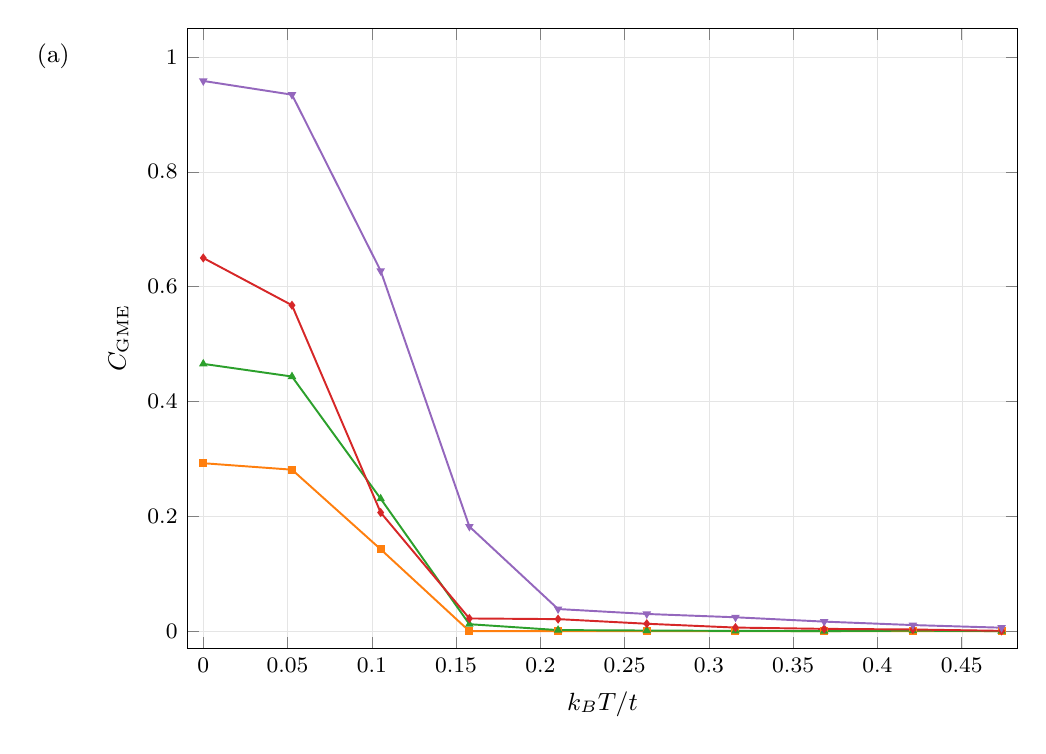
\begin{tikzpicture}
  \begin{axis}[
    width=\columnwidth,
    height=0.78\columnwidth,
    xlabel={$k_B T/t$},
    ylabel={$C_{\mathrm{GME}}$},
    grid=both,
    grid style={line width=.1pt, draw=gray!20},
    tick label style={font=\footnotesize\rmfamily, /pgf/number format/fixed},
    label style={font=\small\rmfamily},
    scaled ticks=false,
    legend style={font=\scriptsize\rmfamily, draw=gray!40, at={(0.5,1.03)}, anchor=south, /tikz/every even column/.append style={column sep=6pt}},
    legend cell align={left},
    legend columns=2,
    ymin=-0.03,
    ymax=1.05,
    xmin=-0.00947368,
    xmax=0.483158,
    after end axis/.append code={\node[anchor=east, font=\small\rmfamily] at (axis description cs:-0.13,0.954) {(a)};},
  ]
    \addplot[color=gmeC1, mark=square*, mark size=1.1pt, line width=0.7pt] coordinates {
        (0,0.292503) (0.052632,0.281207) (0.105263,0.142587) (0.157895,0.000005)
        (0.210526,0.000056) (0.263158,0.000003) (0.315789,0.000006) (0.368421,0.000026)
        (0.421053,0.000002) (0.473684,0)
    };
    \addplot[color=gmeC2, mark=triangle*, mark size=1.1pt, line width=0.7pt] coordinates {
        (0,0.465509) (0.052632,0.443413) (0.105263,0.230654) (0.157895,0.012158)
        (0.210526,0.00188) (0.263158,0.001123) (0.315789,0.000487) (0.368421,0.000099)
        (0.421053,0.000871) (0.473684,0.000093)
    };
    \addplot[color=gmeC3, mark=diamond*, mark size=1.1pt, line width=0.7pt] coordinates {
        (0,0.649928) (0.052632,0.567585) (0.105263,0.206551) (0.157895,0.022128)
        (0.210526,0.020994) (0.263158,0.012923) (0.315789,0.006272) (0.368421,0.004011)
        (0.421053,0.00293) (0.473684,0.000575)
    };
    \addplot[color=gmeC4, mark=triangle*, mark size=1.1pt, mark options={rotate=180}, line width=0.7pt] coordinates {
        (0,0.958182) (0.052632,0.934237) (0.105263,0.627473) (0.157895,0.182198)
        (0.210526,0.038538) (0.263158,0.02995) (0.315789,0.02419) (0.368421,0.016635)
        (0.421053,0.010635) (0.473684,0.006056)
    };
  \end{axis}
\end{tikzpicture}
